\documentclass[crop,tikz]{standalone}


\usetikzlibrary{decorations.pathreplacing}
\usetikzlibrary{arrows}
\begin{document}
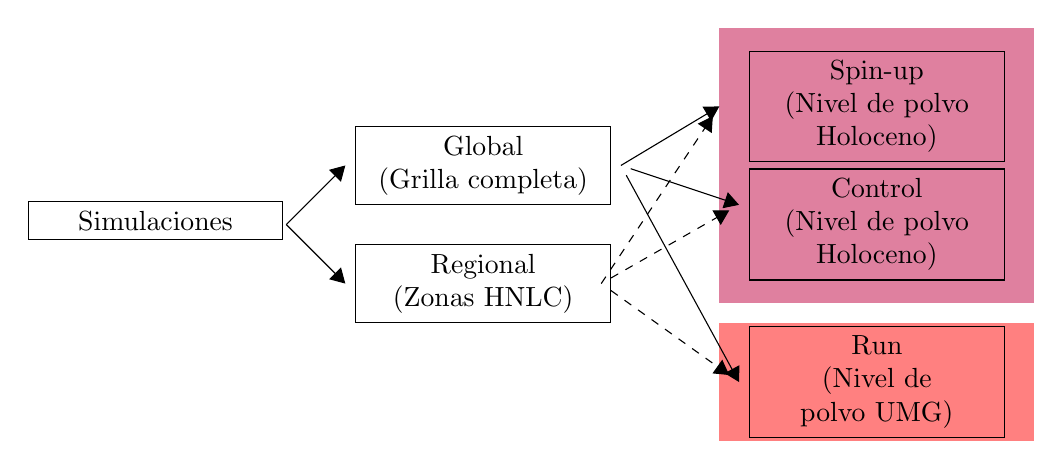
\begin{tikzpicture}
\tikzstyle{nodo texto}=[draw,text width= 3cm,align=center]


\node[nodo texto] at (-4.16,0.3) {Simulaciones };
\node[nodo texto] at (0,1) {Global \\ (Grilla completa)};
\node[nodo texto] at (0,-0.5) {Regional \\ (Zonas HNLC)};

\draw[draw=none,fill=purple!50]  (3,2.75) rectangle (7,-0.75);
\draw[draw=none,fill=red!50] (7,-1) rectangle (3,-2.5);

\node[nodo texto] at (5,1.75) {Spin-up \\ (Nivel de polvo Holoceno)};
\node[nodo texto] at (5,0.25) {Control \\ (Nivel de polvo Holoceno)};
%\node[nodo texto] at (5,0.5) {Run 1 \\ (Nivel de polvo 2)};
%\node[nodo texto] at (5,-1) {Run 2 \\ (Nivel de polvo 3)};
\node[nodo texto] at (5,-1.75) {Run \\ (Nivel de polvo UMG)};


%\node[font=\Huge, sloped] at (5,-2.25) {$\vdots$};

 \draw [-triangle 60](1.75,1) node (v1) {} -- (3,1.75) node (v2) {};
 \draw [-triangle 60](v1) -- (3.25,-1.75) node (v4) {};
 \draw [-triangle 60](v1) -- (3.25,0.5) node (v5) {};
% \draw [-triangle 60](v1) -- (3.25,-1) node (v6) {};
% \draw [-triangle 60](v1) -- (3.25,-2.25);
% \draw [-triangle 60](v1) -- (3.25,-4) node (v7) {};
 \draw [dashed,-triangle 60](1.5,-0.5) node (v3) {} -- (v2);
 \draw [dashed,-triangle 60](v3) -- (v4);
 \draw [dashed,-triangle 60](v3) -- (v5);
% \draw [dashed,-triangle 60](v3) -- (v6);
% \draw [dashed,-triangle 60](v3) -- (3.25,-2);
% \draw [dashed,-triangle 60](v3) -- (v7);
 \draw [-triangle 60](-2.5,0.25) -- (-1.75,1);
 \draw [-triangle 60](-2.5,0.25) -- (-1.75,-0.5);
\end{tikzpicture}
\end{document}
    